% -*- TeX -*-
\documentclass{beamer}

\usepackage{amsmath}
\usepackage{array}
\usepackage{tikz}

\usetikzlibrary{decorations.pathreplacing}
\usetikzlibrary{fit,matrix}

\title{PyLith Modeling Tutorial}
\subtitle{Using Gravity and Stresses}
\author{Charles Williams \\
  Brad Aagaard \\
  Matthew Knepley}
\institute{
\includegraphics[scale=0.4]{../../logos/cig_blackfg}}
\date{June 18, 2016}


% ---------------------------------------------------- CUSTOMIZATION
\newcommand{\thispdfpagelabel}[1]{}
\newcommand{\pylith}[1]{{\color{green}#1}}
\newcommand{\python}[1]{{\color{red}#1}}
\usetheme{CIG}

\newcommand{\tensor}[1]{\overline{#1}}

% ========================================================= DOCUMENT
\begin{document}

% ------------------------------------------------------------ SLIDE
\maketitle

% ------------------------------------------------------------ SLIDE
\logo{
\includegraphics[height=4.5ex]{../../logos/cig_blackfg}}

% ========================================================== SECTION
\section{Gravity Example}
\subsection{Introduction}

% ------------------------------------------------------------ SLIDE
\begin{frame}
  \frametitle{Concepts Covered in this Session}
  \summary{}

  \begin{itemize}
  \item When are gravitational stresses necessary?
  \item Usage of gravitational body forces in 2D
  \item Usage of initial stresses and state variables
  \item Usage of small strain formulation in 2D
  \item Viscoelastic relaxation with a linear Maxwell model
  \item Spatial database with irregular distribution of points in 2D
  \item Turning off elastic prestep for a postseismic simulation
  \end{itemize}

  \vfill
  NOTE:  Accuracy and convergence for gravitational problems will be
  much improved once PyLith includes higher-order elements.
  \vfill
  
\end{frame}


% ------------------------------------------------------------ SLIDE
\begin{frame}
  \frametitle{When Do We Need to Use Gravitational Stresses?}
  \summary{}

  \begin{itemize}
  \item Pressure/stress-dependent rheology
    \begin{itemize}
    \item Pressure-dependent bulk rheology (e.g., plasticity)
    \item Stress-dependent fault rheology (e.g., friction)
    \end{itemize}
  \item Viscoelastic simulations where we care about vertical
    deformation
  \item Other simulations where we care about the absolute stress
    state
  \end{itemize}
  
\end{frame}


% ========================================================== SECTION
\subsection{Overview}

% ------------------------------------------------------------ SLIDE
\begin{frame}
  \frametitle{Gravity Examples}
  \summary{}

  \begin{itemize}
  \item 2-D examples: {\tt\color{red} examples/2d/gravity}
  \begin{itemize}
    \item Steps 1-3: Body forces, initial stresses, infinitesimal strain
      \begin{itemize}
      \item Step 1: Body forces + infinitesimal strain
      \item Step 2: Body forces + infinitesimal strain + initial stress
      \item Step 3: Step 2 + local density variation
      \end{itemize}
    \item Steps 4-7: Body forces, initial stresses,
      finite/infinitesimal strain with postseismic relaxation
      \begin{itemize}
      \item Step 4: Relaxation with infinitesimal strain and no gravity
      \item Step 5: Relaxation with finite strain and no gravity
      \item Step 6: Relaxation with infinitesimal strain and gravity
      \item Step 7: Relaxation with finite strain and gravity
      \end{itemize}
    \item Step 8: Usage of initial state variables and density
      variation
    \end{itemize}
  \item 3-D examples: {\tt\color{red} examples/3d/hex8/step15-17}
  \end{itemize}
  
\end{frame}


% ------------------------------------------------------------ SLIDE
\begin{frame}
  \frametitle{2D Gravity Simulations}
  \summary{Elastic layer over Maxwell viscoelastic layer}

  \begin{center}
    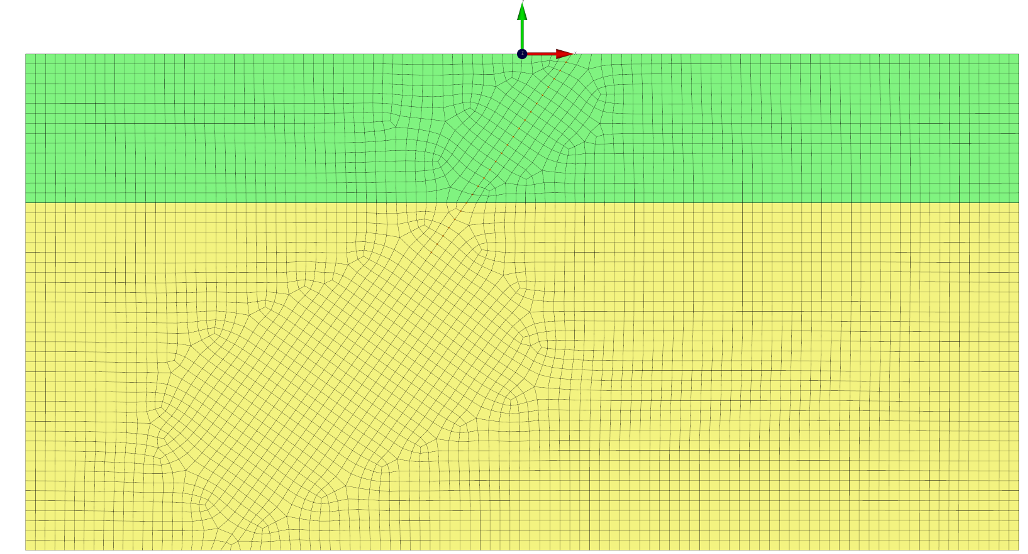
\includegraphics[scale=0.5]{figs/mesh}
  \end{center}
      
\end{frame}


% ========================================================== SECTION
\subsection{Steps 1-3}

% ------------------------------------------------------------ SLIDE
\begin{frame}
  \frametitle{Steps 1-2 in Gravity Example}
  \summary{Infinitesimal strain with and without initial stress}

  \begin{center}
    \begin{tabular}{lc}
      \raisebox{0.48in}{Step01: Infinitesimal strain} &
      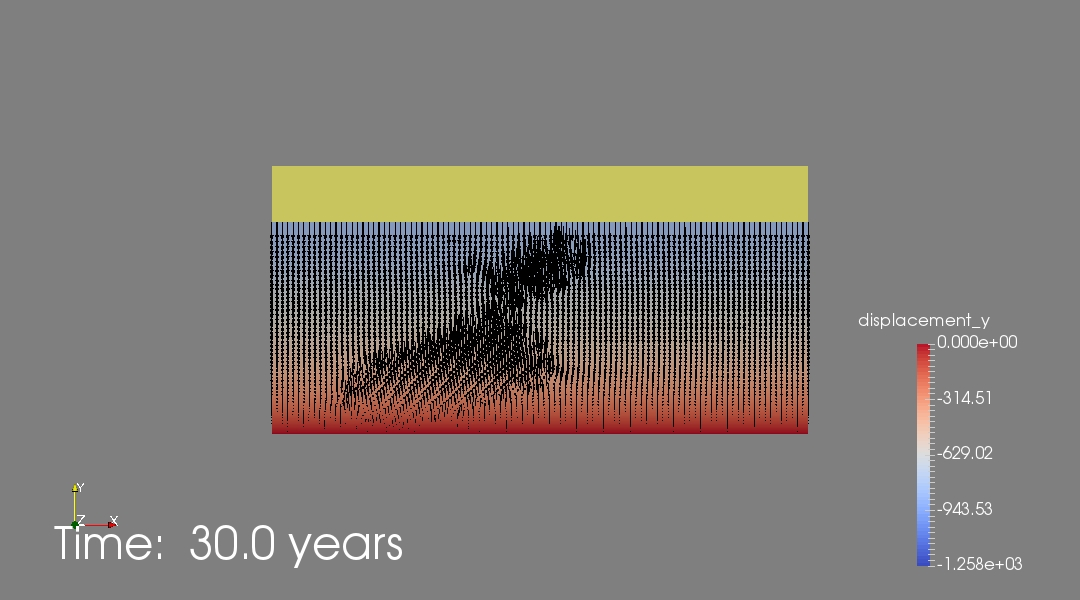
\includegraphics[height=0.95in]{figs/step01} \\
      \raisebox{0.48in}{Step02: Infinitesimal strain + initial stress} &
      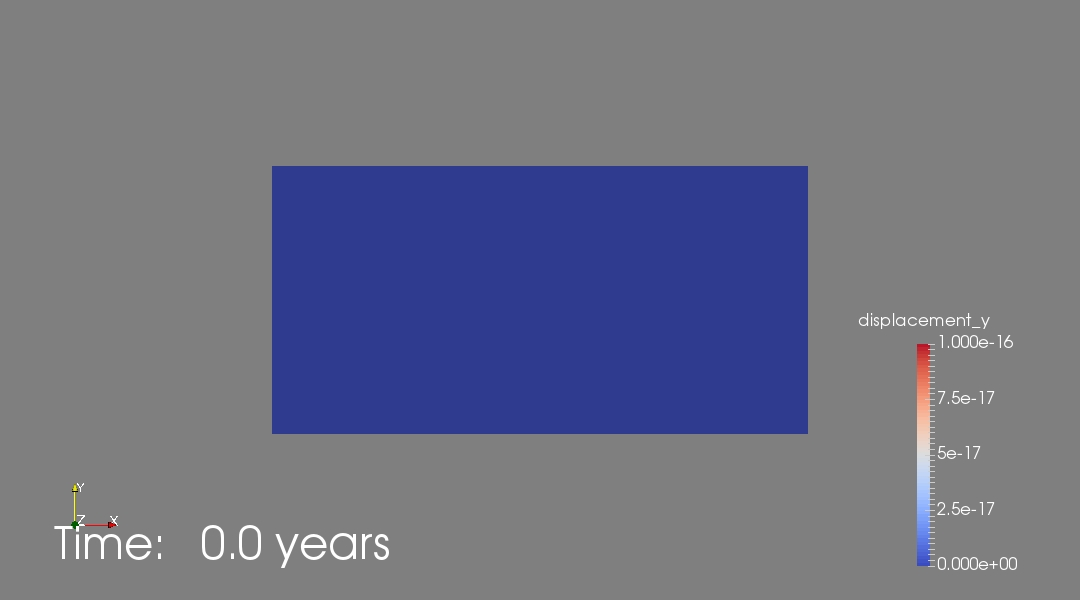
\includegraphics[height=0.95in]{figs/step02} \\
    \end{tabular}
  \end{center}
      
\end{frame}


% ------------------------------------------------------------ SLIDE
\begin{frame}
  \frametitle{Step 3 in Gravity Example}
  \summary{Infinitesimal strain, initial stress, variable density}

  \begin{center}
    \begin{tabular}{lc}
      \raisebox{0.48in}{Density variation} &
      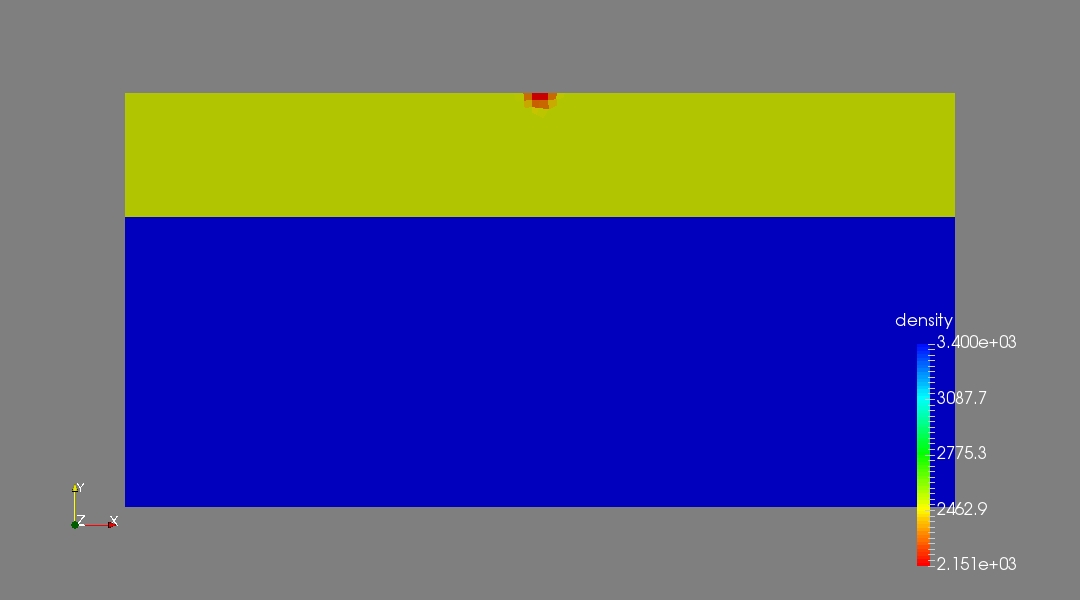
\includegraphics[height=0.95in]{figs/step03-density} \\
      \raisebox{0.48in}{Displacements} &
      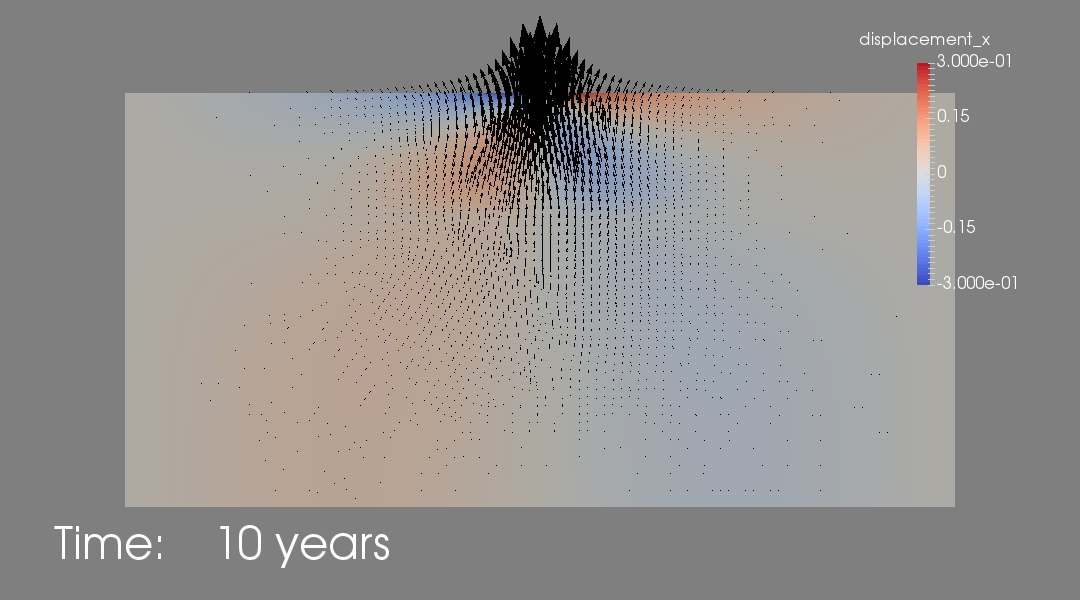
\includegraphics[height=0.95in]{figs/step03} \\
    \end{tabular}
  \end{center}
      
\end{frame}


% ========================================================== SECTION
\subsection{Steps 4-8}

% ------------------------------------------------------------ SLIDE
\begin{frame}
  \frametitle{Postseismic Relaxation Problem Description}
  \summary{Thrust fault plus postseismic relaxation}

  \begin{center}
    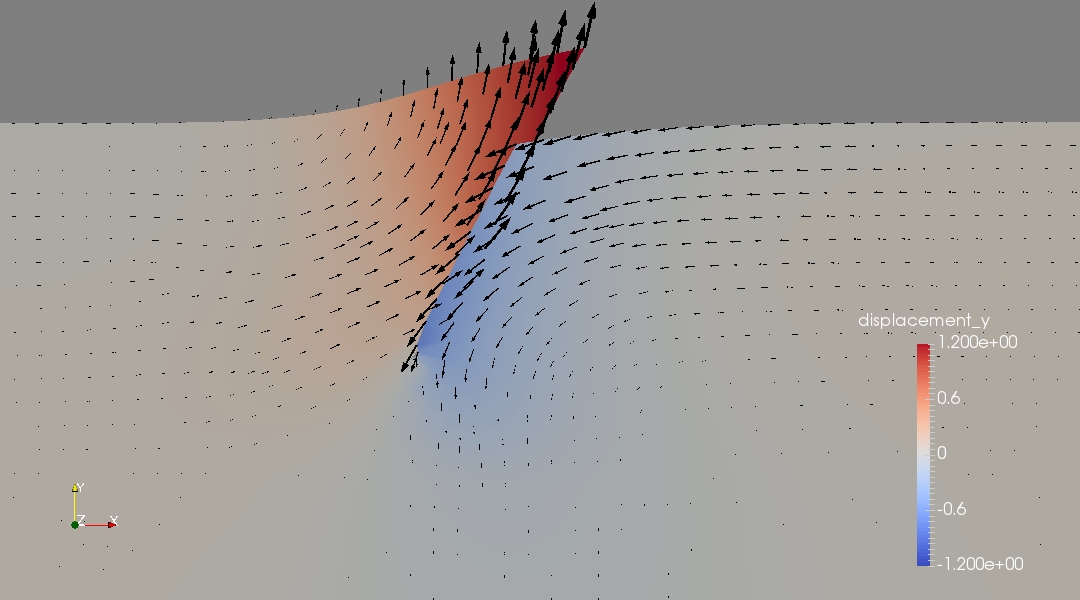
\includegraphics[scale=0.3]{figs/step04-08-descr}
  \end{center}
      
\end{frame}


% ------------------------------------------------------------ SLIDE
\begin{frame}
  \frametitle{Steps 4-7 in Gravity Example}
  \summary{Model differences}

  \begin{center}
    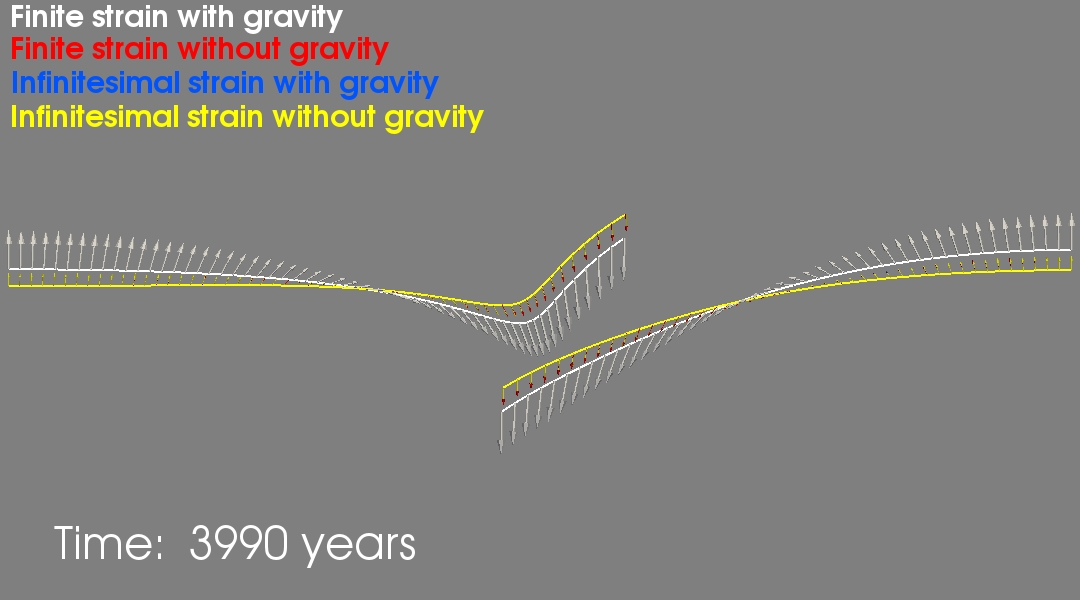
\includegraphics[scale=0.3]{figs/step04-07}
  \end{center}
      
\end{frame}


% ------------------------------------------------------------ SLIDE
\begin{frame}
  \frametitle{Step 8 in Gravity Example}
  \summary{Variable density and initial state variables}

  \begin{center}
    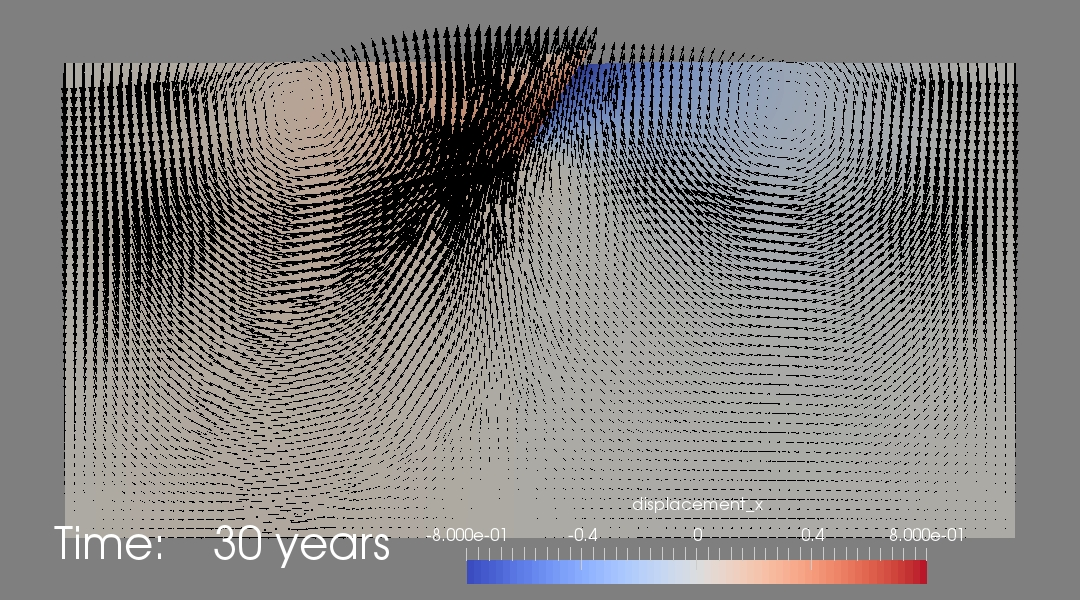
\includegraphics[scale=0.3]{figs/step08}
  \end{center}
      
\end{frame}


% ========================================================== SECTION
\subsection{Files Needed}

% ------------------------------------------------------------ SLIDE
\begin{frame}
  \frametitle{Spatial Databases}
  \summary{}

  \begin{itemize}
  \item {\tt\color{green} matprops\_unidensity.spatialdb} Material properties for
    all simulations except step03 and step08
  \item {\tt\color{green} matprops\_vardensity.spatialdb} Material properties for
    simulations step03 and step08
  \item {\tt\color{green} eqslip.spatialdb} Fault slip for all postseismic
    simulations (step04-step08)
  \item {\tt\color{green} gravity\_isostatic.spatialdb} Isotropic stresses for all
    simulations using initial stresses (step02-step03, step06-step08)
  \item {\tt\color{green} grav\_statevars-xx.spatialdb} State
    variables generated by Python script for step08
  \end{itemize}
  
\end{frame}

% ------------------------------------------------------------ SLIDE
\begin{frame}
  \frametitle{Configuration Files}
  \summary{Settings shared between simulations}

  \begin{itemize}
  \item {\tt\color{green} pylithapp.cfg} Base settings for all
    simulations
  \item {\tt\color{green} postseismic.cfg} Settings for all
    postseismic simulations (step04-step08)
  \item {\tt\color{green} gravity\_initstress.cfg} Settings for all
    simulations using initial stresses (step02-step03, step06-step08)
  \item {\tt\color{green} nogravity.cfg} Settings for all
    simulations without gravity (step04-step05)
  \end{itemize}

  \vfill
  All other {\tt\color{green} .cfg} files are for a specific simulation
  \vfill
  
\end{frame}


% ======================================================================
\end{document}


% End of file
